En función del tipo de la arquitectura de vivienda colectiva (MDU) que se implantará (ver figura~\figref{fig:MDU_Equipment}), el equipo utilizado puede ser similar al empleado en implantaciones OSP o estar especialmente diseñado para el uso interior (véase la ilustración Equipo de MDU de altura elevada-media). El equipo interior está menos sujeto a condiciones ambientales duras y, por tanto, no requiere el mismo grado de robustez que el equipo de planta exterior (OSP).


\begin{wrapfigure}[25]{l}{0.5\textwidth}
  \begin{center}
   	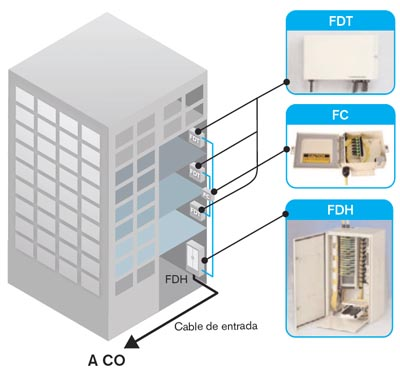
\includegraphics[width=0.5\textwidth]{./img/punto7/Equipo-de-MDU-de-altura-elevada-media.jpg}	
   	\caption{Equipo MDU de altura elevada/media}
	\label{fig:MDU_Equipment}
  \end{center}  
\end{wrapfigure}




Los siguientes elementos se encontrarán normalmente en instalaciones de interior:

Cables de fibra óptica:

\begin{itemize}
\item Los cables de acceso forman el segmento entre la CO y el concentrador de distribución de fibra (FDH) y se encuentran generalmente en el sótano del edificio.
\item Los cables de distribución forman el segmento entre el FDH y el terminal de distribución de fibra (FDT) y se encuentran en cada planta o en el colector de fibra (FC). Los cables de distribución pueden estar formados por una fibra única por puerto divisor o por cables MTP.

\item Los cables de acometida forman el segmento entre el FDT y el ONT y están ubicados en el apartamento. Están generalmente hechos de fibra que es insensible a micro/macrocurvaturas. (Tipo G657)

\end{itemize}

\vfill


\clearpage


Los \textbf{concentradores} de distribución de fibra (FDHs) incluyen:

\begin{itemize}
\item Armarios, cajas de empalmes
\item Divisor(es)
\item Panel(es) de conexiones
\item Elementos de gestión de fibra
\end{itemize}



\textbf{Terminal de distribución} de fibra (FDT):

\begin{itemize}
\item El FDT, ubicado en cada planta, sirve como la conexión entre el FDH y el cable de acometida; puede conectorizarse por fusión (Pigtails) o por conectorización directa (Conectores pre pulidos).
\end{itemize}



\textbf{Colector de fibra} (FC):

\begin{itemize}
\item El FC sirve como un punto de conexión entre el FDH y unos pocos FDTs (ver figura~\figref{fig:Garden_MDU}).
\end{itemize}


\begin{figure}[H]
	\centering
	\includegraphics[width=0.80\textwidth]{./img/punto7/MDU-horizontal-de-estilo-jardín.jpg}
	\caption{MDU horizontal/de estilo jardín}
	\label{fig:Garden_MDU}
\end{figure}


\begin{figure}[H]
	\centering
	\includegraphics[width=0.95\textwidth]{./img/punto7/Enfoques-de-implantación-de-cables-ascendentes-MDU.jpg}
	\caption{Enfoques de implantación de cables ascendentes MDU (aspectos destacados)}
	\label{fig:Ascendant_cables}
\end{figure}



